\section{Proof Strategy}
The claim made by Zhang and Sturton is that a sequence of symbolic execution
trees that abides by the three requirements will yield a set of sequences of concrete
input values, each of which will take the hardware module from the reset state to an
error state.

We prove that if a sequence of trees produced by our abstract Coq model of symbolic
execution, which is based on the three King properties (Properties
\ref{prop:kingsound}, \ref{prop:kingunique}, \ref{prop:kingcommutativity}), abides by
Properties~\ref{prop:startinit}, \ref{prop:correctedz2}, and \ref{prop:stitch}, then
it does yield a set of sequences of concrete inputs that take the abstract Coq model of
concrete execution from the reset state to an error state.




%% Our main correctness theorem that we prove is Theorem \ref{thm:sufficiency}. In other words, given our three property requirements, executing our tree\_list will get us to an error state.


%% We show that given a Coq model of both symbolic execution and the backwards symbolic execution tool and a set of properties, 
%% the backwards symbolic execution tool will give us a list of symbolic execution trees with corresponding leaves that, when executed, will result in an error state.

%% In other words, we define a list of symbolic execution trees, called \textit{tree\_list}, the we bind with a set of properties and a method to execute the relevant leaves, called \textit{execute\_tree\_list},
%% and show that it leads to a set of error states, called \textit{error\_states}. This can be expressed as the following theorem


\begin{theorem}[Correctness of Recursive Strategy]
\label{thm:sufficiency} Consider a sequence of $n$ trees $\mathit{tree\_list} =
\tree_0, \tree_1, \ldots, \tree_{n-1}$, where each tree satisfies King
Properties~\ref{prop:kingsound}-\ref{prop:kingcommutativity}. If
$\mathit{tree\_list}$ satisfies the requirements \ref{prop:startinit},
\ref{prop:correctedz2}, \ref{prop:stitch}, then 
$\mathtt{executeTreeList }(tree\_list) \in error\_states$.
\end{theorem}
 
 In order to prove this, we first prove the following theorem:

\begin{theorem}[Execution ends in leaf of the last tree]
\label{thm:etl}
 $\mathtt{executeTreeList} (tree\_list) \in \mathtt{concretizeLeaf} (\tree)$, where $\tree$ is the last element of $tree\_list$.
\end{theorem}

We then show that $\mathtt{concretizeLeaf} (\tree) \in error\_states$, giving us our result.

We prove Theorem \ref{thm:etl} by induction. 
For our base case, we show that if the list only contains one tree, execution of that tree's root node with input specified by a selected leaf will result in an element of $\mathtt{concretizeLeaf}(\tree)$.

\begin{figure}
\centering
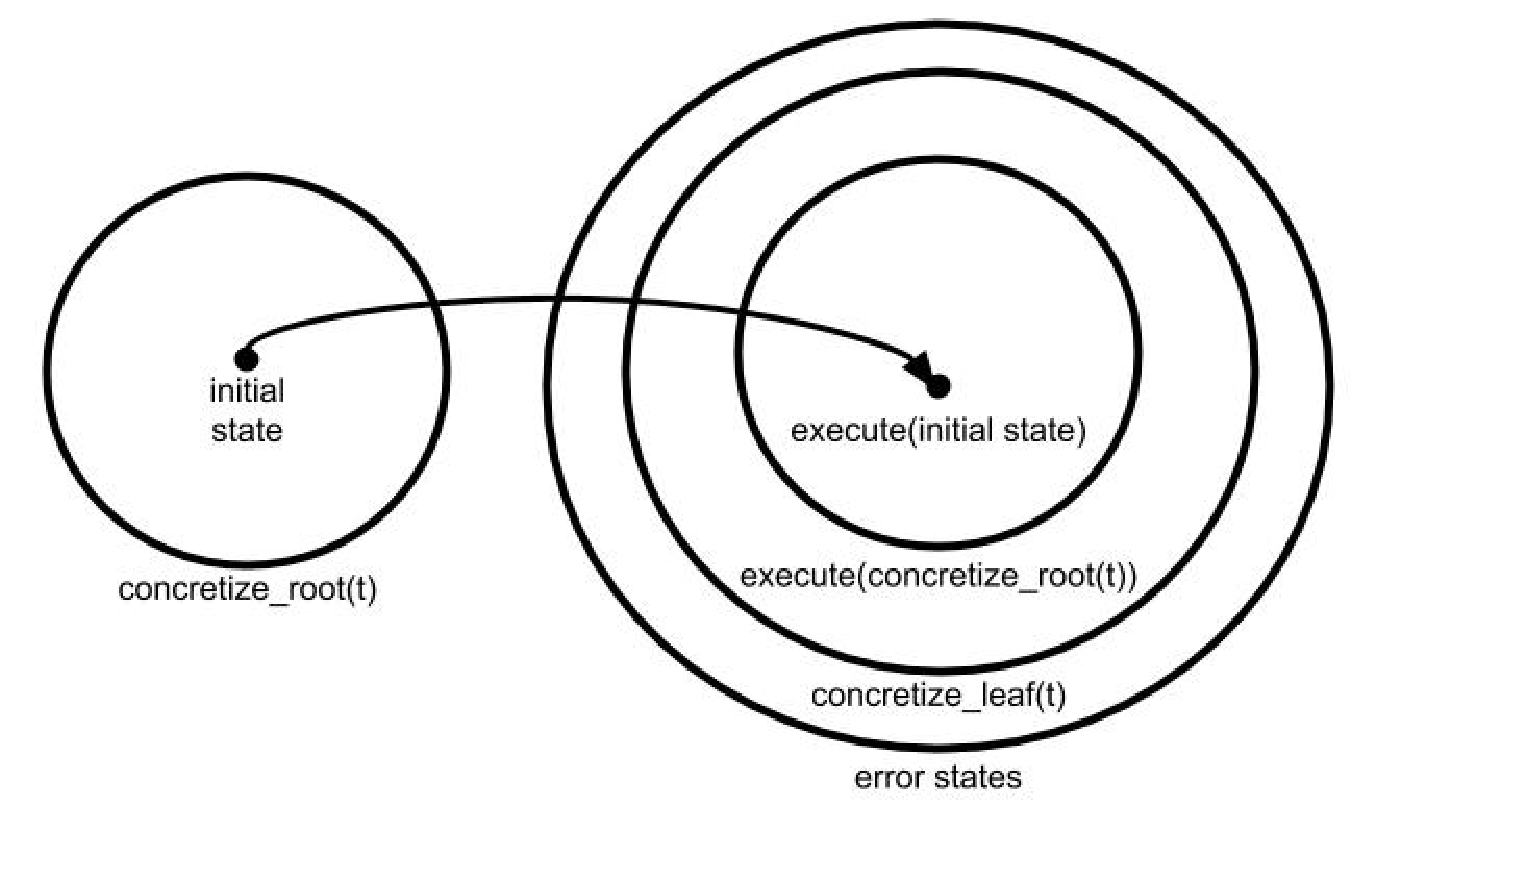
\includegraphics[width=.8\textwidth]{set3.eps}
\caption{Visual depiction of the base case of the proof.}
\label{fig:basecase}
\end{figure}

In other words, as depicted in Figure \ref{fig:basecase}, we show that the initial state is an element of $\mathtt{concretizeRoot}(\tree)$ of the tree \tree, and that concretely executing any element of $\mathtt{concretizeRoot}(\tree)$ will result n an element inside $\mathtt{concretizeLeaf}(\tree).$



For our inductive step, as depicted in Figures  \ref{fig:tlist} and \ref{fig:indstep}, we show that execution of each root with inputs from each specified leaf in a tree list of size $n$ will result in an element of $\mathtt{concretizeLeaf}(\tree_n)$.

Our inductive hypothesis is that $\mathtt{executeTreeList }(tree\_list') \in \mathtt{concretizeLeaf} (\tree_{n-1})$, where $tree\_list'$ is a $tree\_list$ with the last element removed. We then show that $\mathtt{concretizeLeaf} (\tree_{n-1}) \subseteq \mathtt{concretizeRoot} (\tree_{n}) $, and therefore the concrete execution of any element in $\mathtt{concretizeLeaf} (\tree_{n-1}) $ is in the set of of the concrete execution of any element in $\mathtt{concretizeRoot} (\tree_{n})$. Next, we show that $\mathtt{concretizeRoot} (\tree_{n}) \subseteq \mathtt{concretizeLeaf} (\tree_{n})$, giving us our result.
 
\begin{figure}
\centering
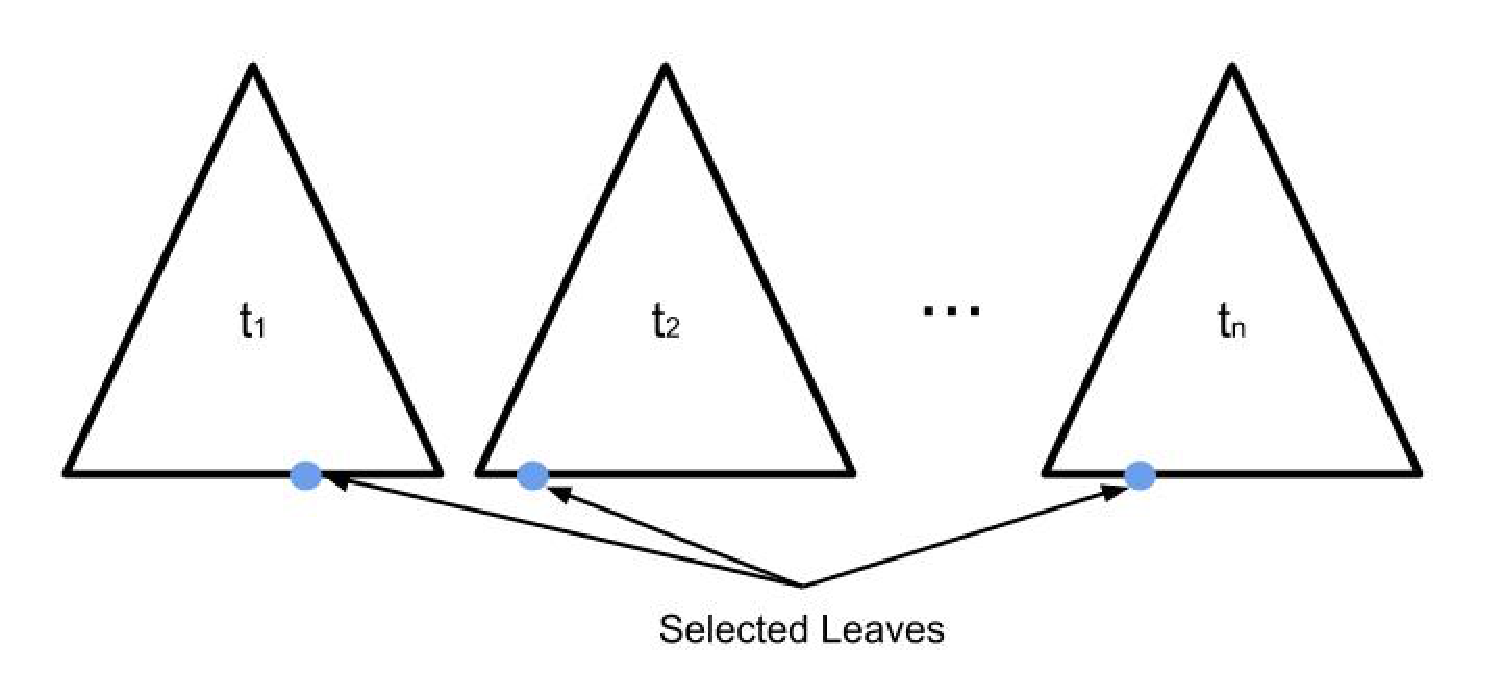
\includegraphics[width=.8\textwidth]{tlist.eps}
\caption{List of trees of length $n$.}
\label{fig:tlist}
\end{figure}

\begin{figure}
\centering
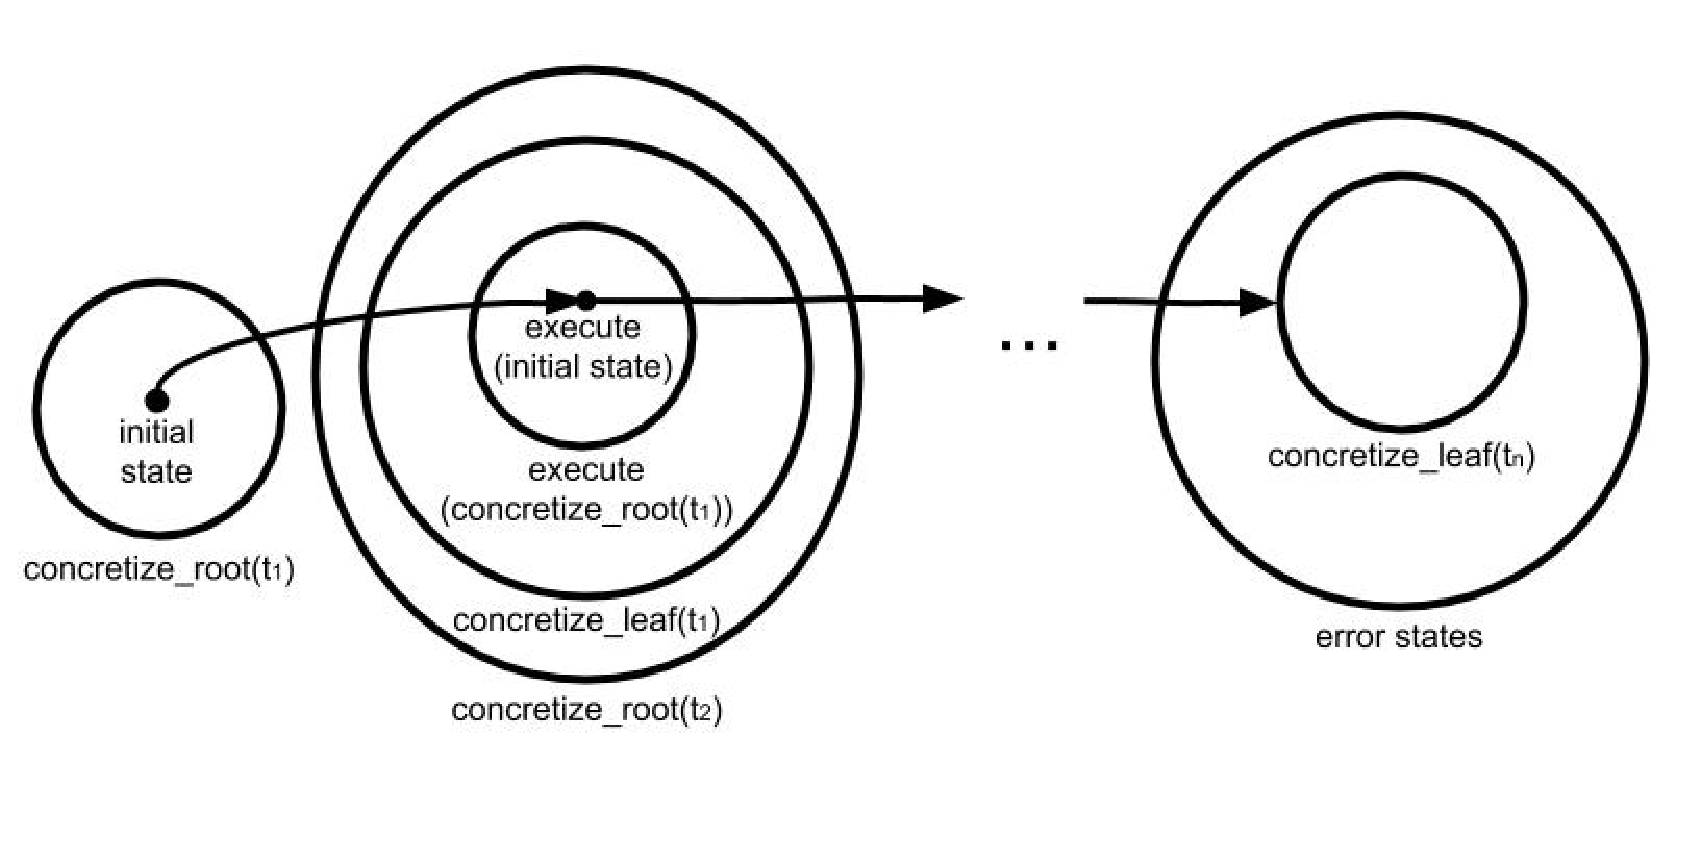
\includegraphics[width=.8\textwidth]{set4.eps}
\caption{Visual depiction of the inductive step of the proof.}
\label{fig:indstep}
\end{figure}




The reason we need \ref{prop:correctedz2} is because \ref{prop:enderror} is not sufficient. 
This is because if $\mathtt{executeTreeList} (tree\_list) \in \mathtt{concretizeLeaf} (\mathtt{last\_element}(tree\_list))$ and \\
$\mathtt{concretizeLeaf} (\mathtt{last\_element} (tree\_list)) \cap error\_states \neq \{\}$, we could get the case where
$\mathtt{executeTreeList} (tree\_list) \notin error\_states$, as shown in Figure \ref{fig:Prop2}.

\begin{figure}
  \centering
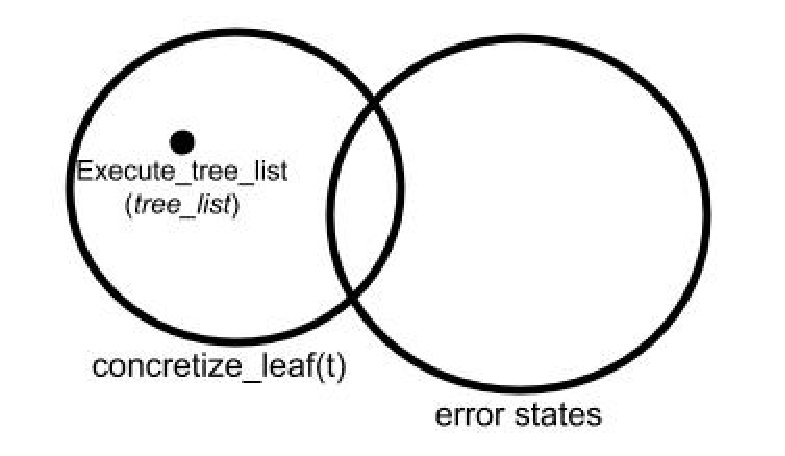
\includegraphics[width=.4\textwidth]{prop2.eps}
\caption{Example of Property $2$ not being sufficient to show $\mathtt{executeTreeList} (tree\_list) \in error\_states$.}
\label{fig:Prop2}
\end{figure}
